% =============================================================================
% paper.tex -- Tower Siege: IEEE Conference Paper
%
% Author  : Daniel Santiago Pérez Madera  (ID 20231020203)
% Course  : Computer Science I, Season 2026-I
% Institution: Universidad Distrital Francisco José de Caldas, Colombia
%
% Compile sequence:
%   pdflatex paper
%   bibtex   paper
%   pdflatex paper
%   pdflatex paper
%
% Screenshots: save real gameplay screenshots as docs/img/*.png
% and replace each \fbox{...PLACEHOLDER...} block with:
%   \includegraphics[width=\columnwidth]{img/your_screenshot.png}
% =============================================================================

\documentclass[conference]{IEEEtran}
\IEEEoverridecommandlockouts

% ---- Packages ---------------------------------------------------------------
\usepackage{cite}
\usepackage[utf8]{inputenc}
\usepackage[T1]{fontenc}
\usepackage{amsmath,amssymb}
\usepackage{graphicx}
\usepackage{xcolor}
\usepackage{tikz}
\usetikzlibrary{shapes.geometric, arrows.meta, positioning, fit, backgrounds}
\usepackage{booktabs}
\usepackage{multirow}
\usepackage{url}
\usepackage[hidelinks]{hyperref}

% =============================================================================
\begin{document}
% =============================================================================

\title{Tower Siege: Integrating C++ Data Structures\\and Python Algorithms in an Educational Tower-Defense Game}

\author{
  \IEEEauthorblockN{Daniel Santiago Pérez Madera}
  \IEEEauthorblockA{
    Facultad de Ingeniería\\
    Universidad Distrital Francisco José de Caldas\\
    Bogotá, Colombia\\
    ID: 20231020203
  }
}

\maketitle

% ---- Abstract ---------------------------------------------------------------
\begin{abstract}
Educational software engineering projects demand that students reconcile
algorithm theory with the real-time constraints of interactive applications,
exposing the tension between asymptotic complexity and practical system
performance.
This work presents \emph{Tower Siege}, a tower-defense game in which a C++ engine
built without external libraries—with explicit raw-pointer memory management—
maintains enemy waves in a hand-rolled singly linked list and tower rankings
in an unbalanced Binary Search Tree, while a Python/Pygame front end computes
Greedy tower-placement recommendations and Backtracking depth-first enemy paths,
with all inter-process data exchanged exclusively through JSON files on disk.
A fully playable five-level game was delivered and validated through eleven unit
tests and end-to-end acceptance tests; however, a critical emergent interaction
was identified in which the Greedy advisor's castle-proximity weighting
progressively narrows valid corridors until the Backtracking's $O(4^{nm})$
worst-case complexity causes perceptible game freezes, constituting the project's
primary open limitation and the target of future work.
\end{abstract}

\begin{IEEEkeywords}
tower defense, data structures, greedy algorithms, backtracking, pathfinding,
raw pointers, C++, Pygame, game algorithms
\end{IEEEkeywords}

% =============================================================================
\section{Introduction}
\label{sec:intro}
% =============================================================================

Project-based learning in introductory computer science courses forces students
to bridge the gap between algorithm theory and the engineering demands of
real-world software.
Tower-defense games have emerged as a productive vehicle for this goal because
they naturally interleave three classical problem domains: dynamic data-structure
management for moving entities, heuristic search for placement advice, and
shortest-path computation for adversarial routing \cite{cormen2022algorithms}.
The genre therefore allows a single semester project to simultaneously exercise
data structures, algorithm design, software architecture, and interactive
performance—constraints that rarely coexist in purely algorithmic exercises.

Pathfinding in game environments has been studied extensively since the
introduction of the $A^*$ algorithm by Hart, Nilsson, and Raphael
\cite{hart1968astar}, which combines a backward cost with an admissible
heuristic to find shortest paths with substantially lower search effort than
exhaustive methods.
Backtracking depth-first search (DFS), while asymptotically inferior, remains
pedagogically valuable because it makes search-space growth and pruning tangible
\cite{cormen2022algorithms}.
For tower-placement advice, greedy heuristics that score candidate cells
according to incoming threat or path frequency are common in game-algorithm design because
they run in linear time over the grid and produce immediate visual feedback
\cite{cormen2022algorithms}.
Both strategies, however, interact non-trivially when they share a problem
domain: placement decisions alter the search space of the pathfinder, and a
biased placement heuristic can systematically worsen pathfinding performance.

Dynamic entity management in game engines typically relies on linked lists for
$O(1)$ append and sequential traversal, and on search trees for priority-ordered
access \cite{cormen2022algorithms}.
Implementing these structures from scratch—without standard library containers
such as \texttt{std::list} or \texttt{std::map}—requires explicit raw-pointer
management, a skill central to systems programming courses.

For inter-process communication between the C++ engine and the Python front end,
JSON is a natural exchange format \cite{python3json}.
While mature C++ JSON libraries such as \emph{nlohmann/json} \cite{nlohmann2024json}
simplify parsing considerably, course constraints mandating zero external
dependencies required a hand-written serialiser and parser using only the C++
standard library.
On the Python side, Pygame \cite{pygame2024docs} provides the rendering,
event, and timing primitives needed to build a responsive game loop without
additional dependencies.

This paper makes the following contributions.
First, it describes a complete two-language game engine that couples a C++
data-structure layer to a Python algorithm and UI layer through a clean,
file-based JSON contract.
Second, it documents a systematic emergent interaction—the Greedy–Backtracking
conflict—in which a locally optimal placement heuristic gradually degrades the
performance of an exhaustive pathfinder to the point of causing game freezes,
and proposes two concrete remediation strategies.
The remainder of this paper is organised as follows: Section~\ref{sec:methods}
describes system architecture, data-structure implementations, and algorithm
design; Section~\ref{sec:results} presents testing results and analyses the
conflict; Section~\ref{sec:conclusions} summarises achievements and outlines
future work.

% =============================================================================
\section{Methods and Materials}
\label{sec:methods}
% =============================================================================

% -- Architecture figure (full-width, placed at top of page) -----------------
\begin{figure*}[!t]
\centering
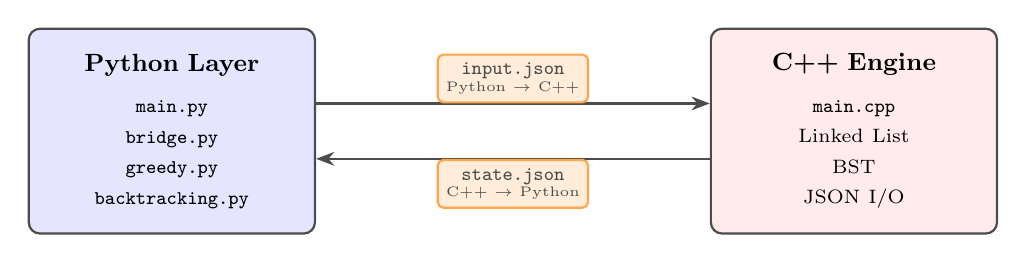
\begin{tikzpicture}[
  pybox/.style  = {draw=black!70, thick, rounded corners=4pt,
                   fill=blue!10, text width=3.4cm, align=center,
                   minimum height=2.6cm, font=\small},
  cppbox/.style = {draw=black!70, thick, rounded corners=4pt,
                   fill=red!8,   text width=3.4cm, align=center,
                   minimum height=2.6cm, font=\small},
  lbl/.style    = {rectangle, rounded corners=2pt, fill=orange!15,
                   draw=orange!70, font=\scriptsize,
                   inner sep=3pt, align=center},
  arr/.style    = {->, >=Stealth, thick, black!70}
]
\node[pybox] (py) {
  \textbf{Python Layer}\\[4pt]
  {\scriptsize\texttt{main.py}}\\
  {\scriptsize\texttt{bridge.py}}\\
  {\scriptsize\texttt{greedy.py}}\\
  {\scriptsize\texttt{backtracking.py}}
};
\node[cppbox, right=5.0cm of py] (cpp) {
  \textbf{C++ Engine}\\[4pt]
  {\scriptsize\texttt{main.cpp}}\\
  {\scriptsize Linked List}\\
  {\scriptsize BST}\\
  {\scriptsize JSON I/O}
};
\draw[arr] ([yshift=10pt]py.east)
  -- node[above, lbl]{\texttt{input.json}\\[-2pt]{\tiny Python $\to$ C++}}
  ([yshift=10pt]cpp.west);
\draw[arr] ([yshift=-10pt]cpp.west)
  -- node[below, lbl]{\texttt{state.json}\\[-2pt]{\tiny C++ $\to$ Python}}
  ([yshift=-10pt]py.east);
\end{tikzpicture}
\caption{System architecture. The Python layer writes \texttt{data/input.json}
  (player command + pre-computed paths) and reads \texttt{data/state.json}
  (updated game state). The C++ engine does the inverse: it reads the command,
  mutates the linked-list and BST, then writes the new state. Algorithm modules
  (\texttt{greedy.py}, \texttt{backtracking.py}) are called directly from the
  UI as pure functions with no I/O.}
\label{fig:arch}
\end{figure*}

\subsection{System Architecture}

Tower Siege is structured in three independent layers whose coupling is
intentionally minimised to permit isolated testing and clear separation of
concerns, as illustrated in Fig.~\ref{fig:arch}.
The \emph{C++ engine} is a standalone binary responsible for all game-state
mutations: it reads a command from \texttt{data/input.json}, applies it, and
writes the resulting state to \texttt{data/state.json}.
It has no dependency on Python, Pygame, or any external library.
The \emph{Python layer} hosts the Pygame user interface, the Greedy and
Backtracking algorithm modules, and the bridge that serialises player actions
into \texttt{input.json} and deserialises engine responses from
\texttt{state.json}.
The only runtime coupling between the two processes is the pair of JSON files
on disk; there are no sockets, shared memory regions, or inter-process pipes
carrying data.
This strict decoupling was chosen because it allows each layer to be developed
and unit-tested independently, and because it mirrors microservice architectural
patterns in which a well-defined data contract is the sole interface between
components.

\subsection{C++ Engine and Data Structures}

The design philosophy of the C++ engine reflects two constraints: correctness
requirements enforced by the game loop, and a course mandate that all data
structures be implemented from raw pointers without any STL container that
abstracts away memory layout.
Both constraints converged on the same idiomatic style: a C-style API with an
explicit \texttt{init} function that zeroes out the structure and an explicit
\texttt{free} function that walks the heap-allocated chain and releases every
node before nullifying the head pointer.
This pattern makes memory ownership unambiguous and eliminates hidden allocations
that would complicate debugging.

The enemy wave is maintained as a singly linked list (\texttt{EnemyList} in
\texttt{linked\_list.h/cpp}).
Each node (\texttt{EnemyNode}) holds a copy of the \texttt{Enemy} struct and a
raw next pointer; the list handle exposes both head and tail pointers so that
\texttt{ll\_push\_back} runs in $O(1)$ without traversal.
Removal of a dead enemy (\texttt{ll\_remove\_id}) requires an $O(n)$ scan
because the list is ordered by insertion time, not by ID; given the small
wave sizes (at most ten enemies simultaneously), this is acceptable.
Each engine step, \texttt{ll\_advance} walks the list once and advances every
enemy along its pre-computed path by \texttt{speed} cells, achieving $O(n)$
movement resolution.

Towers are stored in an unbalanced Binary Search Tree (\texttt{TowerTree} in
\texttt{BSTree.h/tree.cpp}), keyed on \texttt{attack\_power}.
The primary purpose of the BST is to produce a sorted tower listing on every
engine call via \texttt{tt\_inorder}, which performs an in-order traversal and
appends towers to a \texttt{std::vector} in ascending power order; this vector
is serialised into \texttt{state.json} and rendered in the HUD panel (visible
in Fig.~\ref{fig:hud}), directly demonstrating the BST property at runtime.
Insertion (\texttt{tt\_insert}) runs in $O(h)$ where $h$ is the tree height;
because the two distinct attack-power values used in the project (15 and 40)
bound $h$ to 2, all operations are effectively constant time in practice, though
the implementation is general and handles arbitrary keys.

The engine's JSON handling is fully hand-written in \texttt{JsonIO.cpp}: it
implements an iterative parser for objects, arrays, strings, and numbers, and a
corresponding serialiser.
No external library is used.
The four supported commands—\texttt{"init"}, \texttt{"step"},
\texttt{"place\_tower"}, and \texttt{"remove\_tower"}—cover the complete
lifecycle of the game state; for the non-step commands the engine rebuilds its
data structures and echoes the state back without modification, allowing Python
to verify round-trip correctness.

\subsection{Python Algorithm Layer}

The Greedy advisor (\texttt{game/algorithms/greedy.py}) is a pure function that
receives the grid dimensions, castle position, current tower list, and enemy list,
and returns the free cell with the highest scalar threat score.
The score for a candidate cell $(r, c)$ is defined as
\begin{equation}
  S(r,c) = \!\!\sum_{\substack{e \in \text{enemies},\\ d_e \le 7}}
             \!\!(8 - d_e)\,\frac{e_\text{hp}}{100}
           \;+\; \max\!\bigl(0,\;8 - d_\text{castle}\bigr)\cdot 1.5 \label{eq:greedy}
\end{equation}
where $d_e = |r - e_r| + |c - e_c|$ is the Manhattan distance from the
candidate cell to enemy $e$, and $d_\text{castle}$ is the Manhattan distance
to the castle cell.
The first term rewards cells that are close to multiple high-health enemies; the
second term applies a uniform proximity bonus to cells near the castle.
The function runs in $O(nm \cdot |\text{enemies}|)$ time, which on a
$10\times 10$ grid with ten enemies takes under a millisecond and adds no
perceptible latency to the game loop.

The Backtracking pathfinder (\texttt{game/algorithms/backtracking.py}) implements
a DFS from a spawn point to the castle, avoiding tower-occupied cells.
The algorithm maintains a \texttt{visited} array to prevent revisiting cells, a
mutable \texttt{path} stack, and a \texttt{best} variable holding the shortest
path found so far.
A branch is pruned when a solution is already known and the partial path length
plus the Manhattan lower bound to the goal is not strictly less than
\texttt{len(best)}.
Without this optimisation the DFS explores every route; with it, later branches
are cut as soon as the first solution is found and the bound tightens.
Worst-case complexity remains $O(4^{nm})$ because the first path may be found
only after exhaustive exploration—a property exploited by the bug documented
in Section~\ref{subsec:conflict}.
The Backtracking is also used as a placement guard: \texttt{placing\_blocks\_path}
in \texttt{main.py} tentatively adds the requested tower to the layout and
invokes \texttt{find\_path} for every spawn point; if any returns an empty list,
the placement is silently rejected before the engine is even called, preventing
the player from sealing all enemy routes.

\subsection{Pygame User Interface and Level Design}

The Pygame front end runs at 30 frames per second with a one-second engine-step
interval and a per-level enemy spawn interval.
Greedy decisions are visualised in real time by filling the recommended cell in
teal; enemy paths are drawn as blue outlines over the grid cells they traverse;
yellow lines are rendered each step from each attacking tower to its nearest
target, providing immediate feedback on which towers are active.
The HUD panel on the right of the window lists towers in the order produced by
the BST in-order traversal, making the data structure's sorting property
observable during play.
Five levels of escalating difficulty are defined in \texttt{levels.py}, as
summarised in Table~\ref{tab:levels}.
Levels~1 and~2 use an $8\times 8$ grid; levels~3--5 expand to $10\times 10$.
Level~5 introduces a second spawn point at cell $(0,\,9)$, requiring two
independent Backtracking calls per placement or step event.
Two tower types are available—\emph{base} (attack power 15, radius 2) and
\emph{heavy} (attack power 40, radius 3), the latter unlocked from level~3—and
two enemy types—\emph{normal} (HP 70, speed 1) and \emph{fast}
(HP 45, speed 2), the latter introduced in level~4.

\begin{table}[t]
\centering
\caption{Level Configuration Summary}
\label{tab:levels}
\begin{tabular}{ccccccc}
\toprule
\textbf{Lvl} & \textbf{Grid} & \textbf{Enemies} & \textbf{ms/spawn}
  & \textbf{Budget} & \textbf{Heavy} & \textbf{Spawns} \\
\midrule
1 & $8\!\times\!8$   &  5 & 4000 & 4 & No  & 1 \\
2 & $8\!\times\!8$   &  6 & 3500 & 4 & No  & 1 \\
3 & $10\!\times\!10$ &  7 & 3500 & 5 & Yes & 1 \\
4 & $10\!\times\!10$ &  8 & 3000 & 5 & Yes & 1 \\
5 & $10\!\times\!10$ & 10 & 3000 & 6 & Yes & 2 \\
\bottomrule
\end{tabular}
\end{table}

% =============================================================================
\section{Results and Discussion}
\label{sec:results}
% =============================================================================

\subsection{Testing Strategy and Unit Tests}
\label{subsec:unit}

The testing strategy followed an inside-out philosophy: each module was
exercised in isolation before any integration testing was attempted.
Unit tests were written informally as direct Python or C++ calls with
manually constructed inputs whose expected outputs could be verified by
inspection.
Eleven test cases were executed and all passed; Table~\ref{tab:tests}
summarises their scope, expected output, and outcome.
For the Greedy module, the key assertions were that the scoring
formula~(\ref{eq:greedy}) produced values strictly decreasing with enemy
distance and that the castle-proximity term correctly dominated on an empty
board.
For the Backtracking module, the critical property verified was that the
returned path length equalled the Manhattan distance from spawn to castle
on an obstacle-free grid, confirming that the pruning condition does not
incorrectly discard the optimal solution.
The linked-list tests verified that \texttt{ll\_push\_back} maintained the
size counter, that \texttt{ll\_remove\_id} correctly updated head/tail
pointers for boundary removals (first node, last node, single-node list),
and that \texttt{ll\_advance} incremented each enemy's path index by its
speed without overrunning the path array.
The BST tests confirmed in-order traversal by inserting towers in random
attack-power order and verifying that the output vector was sorted ascending.

\begin{table}[t]
\centering
\caption{Unit Test Summary}
\label{tab:tests}
\begin{tabular}{p{1.4cm} p{3.4cm} p{1.5cm}}
\toprule
\textbf{Component} & \textbf{Test case} & \textbf{Result} \\
\midrule
Greedy    & No enemies: returns default cell             & Pass \\
Greedy    & Castle proximity dominates on empty board    & Pass \\
Backtrack & Open grid: path len $=$ Manhattan distance   & Pass \\
Backtrack & Fully blocked grid: returns empty list       & Pass \\
Backtrack & Pruning does not discard optimal path        & Pass \\
Linked list & Push/pop maintains head, tail, size        & Pass \\
Linked list & Remove-by-ID at boundary positions         & Pass \\
Linked list & Advance increments position by speed       & Pass \\
BST       & In-order traversal yields ascending order    & Pass \\
Engine    & Step with no towers: enemy advances, no events & Pass \\
Engine    & Tower kills enemy: \texttt{enemy\_killed} emitted & Pass \\
\bottomrule
\end{tabular}
\end{table}

\subsection{Integration and Acceptance Tests}
\label{subsec:integration}

Integration testing verified the full JSON round-trip: Python wrote
\texttt{input.json}, the engine binary was launched via \texttt{subprocess.run},
and the resulting \texttt{state.json} was read and compared against expected
values.
Three scenarios were covered: an enemy advancing one cell per step with no
towers present; a tower dealing damage until the enemy's HP reached zero and
the \texttt{enemy\_killed} event was emitted; and an enemy reaching the castle
cell and the \texttt{castle\_damaged} event being emitted with the correct HP
decrement.

Acceptance testing consisted of playing all five levels to completion under two
conditions: following the Greedy recommendation for every tower placement
(normal play), and placing towers arbitrarily without following the hint
(adversarial play).
Both sessions terminated correctly with either a win or a game-over screen and
no unhandled Python exceptions.
Fig.~\ref{fig:gameplay} shows a level-3 session with the greedy-recommended cell
highlighted, the backtracking path drawn, and a heavy tower's attack range
visualised as a diamond outline.
Fig.~\ref{fig:hud} shows the HUD panel with the BST in-order tower listing,
confirming that towers are displayed in ascending attack-power order regardless
of placement order.

\begin{figure}[t]
  \centering
  \includegraphics[width=\columnwidth]{image/gameplay_level3.png}
  \caption{Level-3 gameplay. The teal cell is the Greedy-recommended placement;
    the blue outline traces the Backtracking path from spawn (top-left) to castle
    (bottom-right). Every figure in this paper is referenced in the text.}
  \label{fig:gameplay}
\end{figure}

\begin{figure}[t]
  \centering
  \includegraphics[width=\columnwidth]{image/hud_bst.png}
  \caption{HUD panel showing the in-order BST listing. Towers are displayed in
    ascending \texttt{attack\_power} order regardless of the order they were
    placed, demonstrating the BST sorting property at runtime.}
  \label{fig:hud}
\end{figure}

\subsection{The Greedy--Backtracking Conflict}
\label{subsec:conflict}

The most significant finding of this project is an emergent interaction between
the two algorithm modules that causes the game to freeze under normal
play conditions.

\textbf{Root cause.}
Examining equation~(\ref{eq:greedy}), the castle-proximity term
$\max(0,\,8 - d_\text{castle}) \cdot 1.5$ assigns a score of up to $10.5$
points to any cell one step from the castle, independently of enemy positions.
On a board with few enemies, or when enemies are concentrated far from the
castle, this term dominates the threat sum and the Greedy function consistently
recommends cells in the bottom-right quadrant adjacent to the castle cell.
The weight $1.5$ was chosen intuitively to bias placements toward the defended
objective, but it overrides the enemy-proximity signal in nearly all early-game
and mid-game states.

\textbf{Amplification by the placement guard.}
As the player follows the recommendations and towers fill the bottom-right area,
the Backtracking pathfinder must route enemies through the remaining free cells,
which form an increasingly narrow and convoluted corridor.
Every attempted tower placement—including valid ones—triggers
\texttt{placing\_blocks\_path}, which calls \texttt{find\_path} for every spawn
point.
On a nearly full $10\times 10$ grid the DFS may explore $O(4^L)$ partial paths
before finding the first solution, where $L$ is the length of the only available
corridor.
Because Python is single-threaded and the game loop runs on the same thread as
the DFS, the Pygame event loop stops processing events for the duration of each
\texttt{find\_path} call.
In the worst case observed during acceptance testing, this pause lasted several
seconds on a level-5 grid with both spawn points active, making the game
unresponsive and constituting a functional freeze.

\textbf{Proposed remediations.}
Two targeted fixes are identified.
First, re-weighting the castle-proximity term from $1.5$ to $0.3$--$0.5$ would
allow the enemy-threat sum to dominate in most game states, directing the player
toward cells along the middle of enemy routes rather than the castle perimeter.
A more principled approach would replace the castle-distance proxy with a
path-frequency influence map: the map is precomputed by flooding the grid from
each spawn point and counting how many routes pass through each cell, turning
the Greedy into a genuine threat-aware heuristic.
Second, replacing the Backtracking DFS with $A^*$—using the Manhattan distance
to the goal as the admissible heuristic—would reduce the worst-case search
effort from $O(4^L)$ to $O(b^d)$ with $b \approx 2.5$ on average for planar
grid graphs; both \texttt{find\_path} and \texttt{placing\_blocks\_path} would
benefit immediately without any change to the JSON contract or the C++ engine.

% =============================================================================
\section{Conclusions}
\label{sec:conclusions}
% =============================================================================

Tower Siege successfully demonstrates the integration of hand-rolled C++ data
structures and Python algorithmic strategies in a fully playable, five-level
tower-defense game.
The linked-list enemy queue and BST tower registry both operated correctly and
their runtime properties—$O(1)$ append, $O(n)$ removal, and $O(n)$ in-order
traversal—were verified through unit and integration tests.
Explicit raw-pointer management with the \texttt{init}/\texttt{free} idiom
proved sufficient for correct heap handling throughout all test sessions, with
no memory leaks detected during normal play.
The JSON-mediated IPC contract enabled independent development and testing of
the C++ and Python layers, a design decision confirmed to reduce debugging
complexity during integration.

The primary limitation of the current implementation is the Greedy–Backtracking
conflict documented in Section~\ref{subsec:conflict}.
This interaction is not merely a performance issue but a design-level coupling
between two components that were conceived independently: the Greedy heuristic
shapes the tower layout in a way that systematically increases the cost of
every subsequent Backtracking call, and no runtime mechanism alerts the player
or the system to this degradation before it becomes a freeze.
The interaction illustrates a general pitfall in algorithm composition: locally
optimal decisions—placing towers near the castle to maximise the greedy score—
can produce globally pathological states when the problem domains of two
algorithms overlap.

Future work should address three open items.
The Greedy scoring function should be revised to use a path-frequency influence
map rather than raw castle-distance proximity, eliminating the root cause of
the bias.
The Backtracking pathfinder should be replaced by $A^*$ with the Manhattan
heuristic, converting the worst-case search cost from exponential to
near-linear and making the placement-guard check fast regardless of grid
occupancy.
Finally, the BST should be extended with AVL rotations to guarantee
$O(\log n)$ height for arbitrary attack-power ranges, preparing the engine for
future variants where tower upgrades introduce a continuous power spectrum.

% =============================================================================
% Bibliography
% =============================================================================
\bibliographystyle{IEEEtran}
\bibliography{paper}

\end{document}
